\section{Desarrollo de Serious Game} \label{sec:desarrollo}

Según \cite{education:games} un buen videojuego basado en el aprendizaje debe cumplir  los siguientes tres criterios:

\begin{itemize}
\item \textbf{Implementación técnica:} actividad de programación y ejecución de un patrón de diseño. Incluye la perfecta integración de los elementos de diseño en el juego.
\item \textbf{Adecuación para la educación:} la capacidad del juego para hacer frente a las metas curriculares o educativas y la habilidad o el conocimiento del jugador relativo a los contenidos educativos que se aborde.
\item \textbf{Integración total con los objetivos:} la integración del patrón de diseño y el juego en general con los objetivos educativos.
\end{itemize}

En esta sección se describen las dimensiones que deben considerarse para los videojuegos basados en  aprendizaje y las puntos que deben tenerse en cuenta en el diseño y desarrollo  de un serious game. 


\subsection{Dimensiones para los videojuegos basados en aprendizaje}

Las cuatro dimensiones que deben considerarse en el desarrollo de videojuegos educativos son las  siguientes\cite{education:games}:

\begin{itemize}
\item \textbf{Contexto:} es decir, donde ocurre el aprendizaje, lo que va desde aspectos macro, como  factores políticos, económicos e históricos, hasta aspectos micro como la experiencia y  antecedentes de los profesores, costos de licencia, entre otros.
\item \textbf{Tipo de aprendizaje:} para el individuo o grupo, requiere que se considere su  estilo de aprendizaje y sus conocimientos previos, y qué métodos se ajustan mejor a sus  necesidades.
\item \textbf{Modo de representación:} lo que incluye el nivel de interactividad requerido, la fidelidad y  el nivel de inmersión producido. Además cubre la narración de los hechos, la separación de los  aspectos de inmersión con la reflexión de haber utilizado el videojuego. Y de manera importante  enfatiza el potencial de retroalimentación que refuerza el aprendizaje.
\item \textbf{Principios pedagógicos:} es necesario que se reflexione sobre los modelos de aprendizaje lo  que permite producir apropiados planes de lecciones.
\end{itemize}

Estos aspectos o dimensiones no pueden ser consideradas individualmente, todas estas relacionadas  como se muestra en el figura~\ref{fig:desarrollo_dimensiones}.

\begin{figure}[H]
\centering
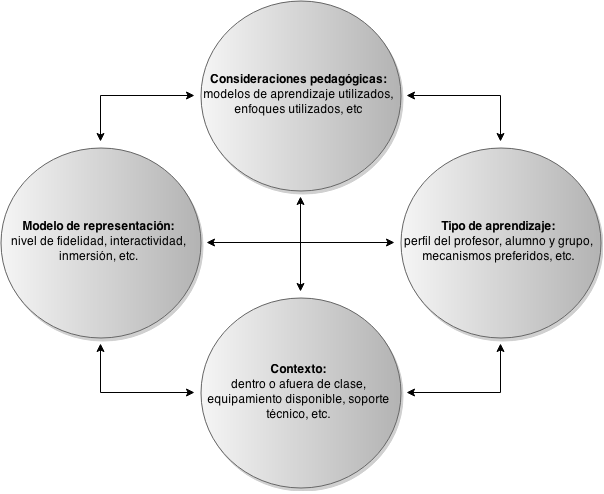
\includegraphics[scale=0.5]{juegos_serios/desarrollo_dimensiones.png}
\caption{Relación entre las cuatro dimensiones a considerarse en un videojuego basado en aprendizaje}
\label{fig:desarrollo_dimensiones}
\end{figure}

Considerando estas dimensiones, a continuación se muestra un ejemplo de flujo de diseño basado en un juego serio desarrollado.


\subsection{Flujo (Living Forest)}


Pereira\cite{pereira2009design} en el diseño del juego \emph{Living Forest} utiliza los pasos definidos a continuación como modelo de creación de un juego serio a partir de la definición previa de las competencias básicas que se desean enseñar.

Primero se definen las competencias básicas y luego se diseña y desarrolla el juego. A continuación la figura~\ref{fig:tics_flujo_diseño_prop} muestra el proceso de desarrollo y luego se explica cada ítem.

\begin{figure}[ht!]
\centering
\begin{tikzpicture}[auto]
    % Place nodes
    \node [block] (1) {Objetivos de diseño};
    \node [block, right of=1, node distance=5cm] (2) {Competencias básicas relacionadas con la educación};
    \node [block, right of=2, node distance=5cm] (3) {Investigación del dominio};
    \node [block, below of=3, node distance=3cm] (4) {Diseño del juego};
    \node [block, left of=4, node distance=5cm] (5) {Tiempo en el juego};
    \node [block, left of=5, node distance=5cm] (6) {Acciones de jugabilidad};
    \node [block, below of=6, node distance=3cm] (7) {Indicadores};
    \node [block, right of=7, node distance=5cm] (8) {Representación e interacción};
    \node [block, right of=8, node distance=5cm] (9) {Implementación};
    \node [block, below of=9, node distance=3cm] (10) {Evaluación};
    % Draw edges
    \path [line] (1) -- (2);
    \path [line] (2) -- (3);
    \path [line] (3) -- (4);
    \path [line] (4) -- (5);
    \path [line] (5) -- (6);
    \path [line] (6) -- (7);
    \path [line] (7) -- (8);
    \path [line] (8) -- (9);
    \path [line] (9) -- (10);
\end{tikzpicture}

\caption{Flujo de diseño propuesto de un Serious Game}
\label{fig:tics_flujo_diseño_prop}
\end{figure}


\subsection{Partes del flujo de diseño}

A continuación se describen cada una de las partes mencionadas
en~\ref{fig:tics_flujo_diseño_prop}.

\subsubsection{Objetivos de diseño}

Definen cuál es el propósito del juego, donde se toman en cuenta los objetivos pedagógicos, así como también objetivos que garanticen que el mismo sea agradable, intuitivo y motivador.

\subsubsection{Competencias básicas relacionadas con la educación} 

Se identifican aquellas que influyen en el diseño del juego, se definen los conocimientos mínimos que se desea que tenga un usuario que lo utilice.

Las competencias básicas pueden tener diferentes orígenes, en el ámbito académico se pude utilizar el plan de estudios, en una empresa se pueden utilizar los objetivos y la visión de la misma.

\subsubsection{Investigación del dominio}

Esta fase se encarga de recabar información exacta acerca del dominio en el cual se desenvuelve el juego serio, en esta fase es importante que participe un experto en el dominio, por ejemplo, en el ámbito académico se puede contar con un profesor experto en el dominio.

Es importante realizar la pregunta \emph{¿Que nivel de detalle es necesario?}, para así definir que contenido incluir, y que factores se deben analizar.

Además es necesario investigar las acciones que se podrían realizar dentro del juego, como se desenvolverá el jugador, por cada acción definida, se deben analizar los elementos y factores relacionados que se deben modelar.

\subsubsection{Diseño del juego}

A partir de la idea original y basado en la información recogida se determina el papel desempeñado por el jugador (de acuerdo a la semántica y pragmática de las acciones y decisiones que está llamado a hacer). 

Se define el nivel de aproximación a la realidad, el nivel de detalle del entorno, del jugador y de las acciones.

Otro factor que se debe tener en cuenta en esta fase es la cantidad de tiempo que pasará un jugador en el juego, se deben modelar todas las acciones del jugador y el entorno de acuerdo a este tiempo.

\subsubsection{Tiempo de juego}

El primer factor que se debe estudiar es el período de adaptación del jugador, lo que depende de la intuitividad del juego, este tiempo debe ser analizado por separado a la hora de realizar un análisis de los resultados.

Si el juego tiene una duración reducida, se tienen que analizar mecanismos para mostrar los resultados de las decisiones a largo plazo, además de como mostrar los resultados de las acciones de corto plazo.

\subsubsection{Indicadores}

Es todo aquello que muestre información relevante al jugador acerca de su estado, ejemplos de este tipo de indicadores son el puntaje, tiempo empleado, objetivos cumplidos. 

La definición de como se juzgará la calidad de una partida del jugador debe ser definida, normalmente mediante un puntaje general, el mismo debe mostrar claramente los resultados de las acciones, si las mismas fueron positivas o negativas para el logro final de los objetivos.

\subsubsection{Representación e interacción}

Representación se refiere a como se visualiza el entorno, e interacción como se relaciona el jugador con su entorno.

Se inicia con un bosquejo de las representaciones de la escena del juego, para así poder definir los elementos que forman parte de la escena.

Otros bosquejos necesarios son los del concepto que se modela en la lógica del juego, para así definir las animaciones del entorno y del jugador.

Se debe definir las alertas sonaras, qué partes del entorno produce sonidos, cómo el jugador recibe estas alertas (por ejemplo si el origen de las mismas es siempre el mismo o importa la distancia a la cámara), se puede agregar música de ambiente si el juego lo amerita.

Se define la interfaz del usuario, qué información será representada, las acciones disponibles desde la misma, además se define si el mismo será en primera persona (la cámara son los ojos del jugador) o en tercera persona (la cámara se sitúa inmediatamente atrás y arriba de la cabeza), como será la interacción con la cámara, acercamientos y movimientos para contemplar el entorno.

\subsubsection{Implementación} 

En esta etapa se estudia el estado del arte de las plataformas tecnológicas disponibles para el desarrollo del juego, se toman en cuenta los factores como la disponibilidad de componentes, de documentación, lenguajes de programación y herramientas de pruebas automáticas.

El proceso puede ser iterativo, entre sesiones de implementación y evaluación de lo implementado, para así poder realizar optimizaciones enfocadas especialmente en la estética, la retroalimentación y el estado del jugador.

\subsubsection{Evaluación} 

Durante el desarrollo del juego serio, se deben realizar varias sesiones de evaluación, por ejemplo, con los responsables o expertos y miembros de la audiencia objetivo. Así mismo, se debe realizar evaluaciones con los grupos de interés las cuales se centra en la adaptación del juego (usabilidad). 

La primera se centra en la validación del modelo de la simulación (refinamiento), mientras que la segunda evaluación sirve para probar el juego en un escenario (parecido al final) y evaluar los aspectos relacionados con el proceso de aprendizaje.  